\documentclass[thesis.tex]{subfiles}

\title{Estimating duration in the presence of misclassification}
\author{Joshua Blake}
\date{\today}

\begin{document}

\ifSubfilesClassLoaded{
  \setcounter{chapter}{5}
}

\chapter{Survival analysis with false negatives} \label{imperf-test}

\todo[inline]{The first paragraph needs restructuring. Dani will send some ideas.}
In \cref{E-perf-test}, a framework for analysing the CIS to produce estimates of the duration of positivity was developed.
However, initial application of this framework produced implausibly short estimates; I identified the issue as being due to the presence of false negatives, a form of misclassification bias, within the CIS (\cref{imperf-test:sec:problem}).
There exists little prior work on the incorporation of misclassification bias within similar survival analysis frameworks.
\todo[inline]{Review literature properly, here or elsewhere}
In this chapter, I modify the previous model to include false negatives (\cref{imperf-test:sec:modelling}).
I show in simulation that this model will recover the duration distribution (\cref{imperf-test:sec:sim-study-results}) and apply it to the CIS data (\cref{imperf-test:sec:application}).
Finally, I discuss the results and further work in \cref{imperf-test:sec:discussion}.

{\color{red}{NEW BIT}}
In \cref{E-perf-test}, a framework for analysing the CIS to produce estimates of the duration of positivity was developed.
However, initial application of this framework produced implausibly short estimate. In this chapter I identify this issue to be the result of false negatives, a form of misclassification bias, within the CIS (\cref{imperf-test:sec:problem}).  In \cref{imperf-test:sec:modelling} I develop the model in \cref{E-perf-test} to include the possibility of observing false negatives.
There exists little prior work on the incorporation of misclassification bias within similar survival analysis frameworks.
\todo[inline]{Review literature properly, here or elsewhere}. Building on this literature, model adaptation to include false negatives involves.....GIVE DETAILS OF WHAT YOU DID
After showing through simulation (\cref{imperf-test:sec:sim-study-results}) that the new model recovers the true duration distribution (\cref{imperf-test:sec:sim-study-results}),  and I apply it to the CIS data (\cref{imperf-test:sec:application}).
Finally, I discuss the results and further work in \cref{imperf-test:sec:discussion}.


\section{The problem} \label{imperf-test:sec:problem}

Applying the method of \cref{E-perf-test} to CIS data estimates fewer individuals of a duration less than three weeks, compared to \cref{E-ATACCC} (see \cref{imperf-test:fig:problem-cis-estimates}).
The \cref{E-ATACCC} estimates are more reliable over the first 2--3 weeks due to them having dense data collection here.
This suggests an issue in the estimation using CIS data.
\begin{figure}
  \centering 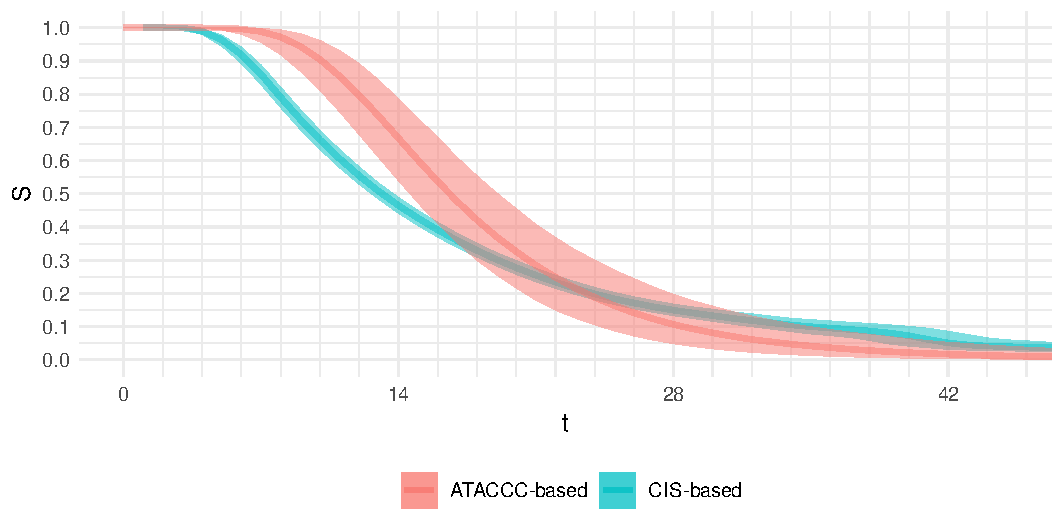
\includegraphics{cis-imperfect-testing/CIS_perfect}
  \caption[Estimating survival using CIS data assuming perfect testing]{Estimates of the survival function using CIS data alongside the ATACCC-based estimates of \cref{E-perf-test}. CIS-based has more episodes ending in the first 14 days. \label{imperf-test:fig:problem-cis-estimates}}
\end{figure}

Comparing repeated data simulations using the setup of \cref{E-perf-test:sec:simulation-study} to the observed CIS data, suggests that this is due to the high frequency of single positive episodes in the CIS data (compare the histogram with $\psens=1$ and the vertical line in \cref{imperf-test:fig:sim-single-pos}).
A single positive episode is an episode containing exactly one positive test; intuitively, these cause estimates to be shorter because the lower bound on the length of time the episode is 1 day, the shortest possible.
Specifically, if $i$ is a single positive episode then $i$'s admissible region (as defined in \cref{E-perf-test:sec:model}) includes $b_i = e_i = r_i^{(b)} = l_i^{(e)}$.
In this case, the beginning and end day of the episode are both equal to the day of this one positive test.
If this is true, then the duration is $d_i = e_i - b_i + 1 = 1$.
Additionally, short episodes are very likely to be missed, which means that the design of the CIS cannot rule out many of them occurring.
% This produced the same pattern, that is estimating too many short episodes (not shown).

\Textcite{shenNonparametrica}, extending \textcite{panNote}, studied the situation when only the terminating event is interval censored and the initiating event has simple left truncation.
They showed that the maximum likelihood estimator is inconsistent if there is at least one single positive episode\todo{check the precise results and condition} and can lead to a severely biased underestimation of the survival function.
The CIS is a more complex setting, including double interval censoring and a complex pattern of missed episodes (see \cref{E-perf-test:sec:problem}).
This means the result cannot simply be extended to the CIS, but still reinforces the intuition that single positive episodes are likely to be problematic.

% Discussion and interrogation of the data led me to
I hypothesised that the reason for the unexpectedly high number of single positive episodes (compared to simulation) was the presence of false negative results.
There are several strands of evidence supporting this hypothesis.
First, it is well known that RT-PCR testing can return false negatives  (see \cref{E-biology-data:sec:PCR}); I explicitly include them in the viral load model of \cref{E-ATACCC}.
Intermittent negatives (described in  \cref{E-biology-data:sec:PCR}) show that they occur within the CIS.
Furthermore, in \cref{imperf-test:sec:simulate}, I expanded the simulation study of \cref{E-perf-test:sec:simulation-study} to include false negatives (see  for more details).
This reproduced the CIS data more faithfully and exhibited the same issues when estimating the duration distribution (see \cref{imperf-test:fig:sim-single-pos}).
\begin{figure}
  \centering 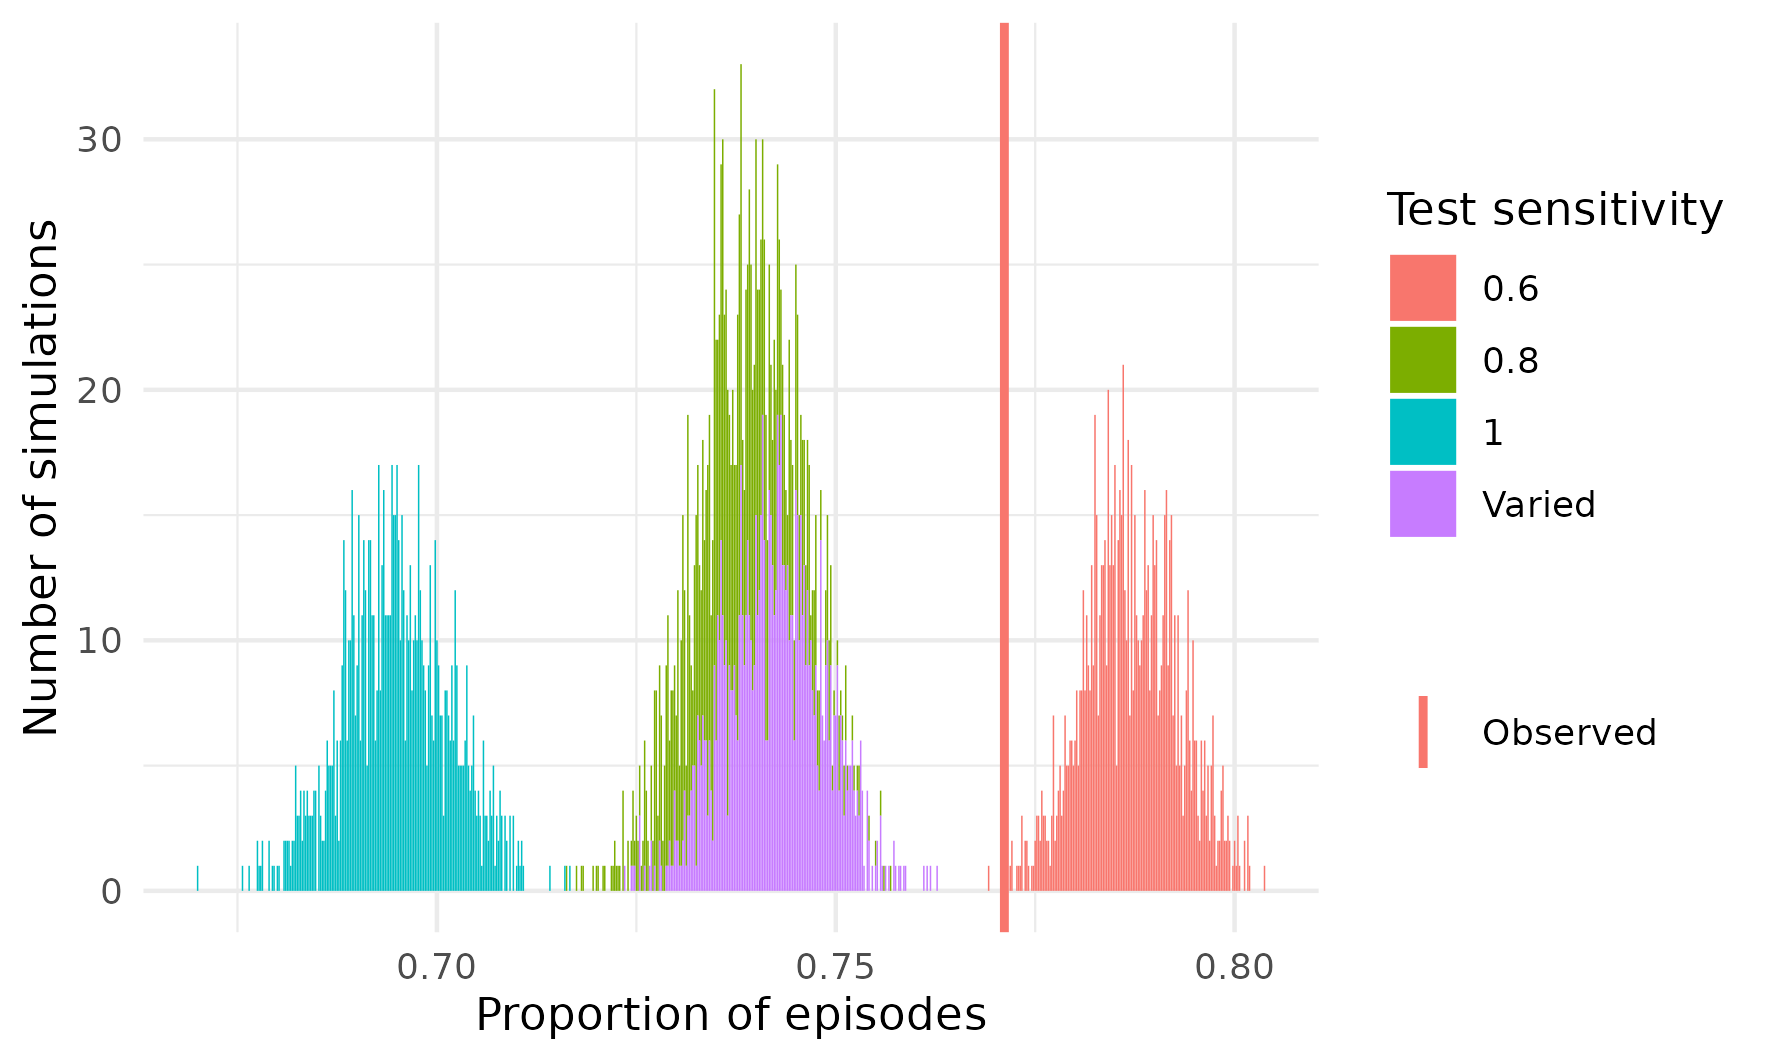
\includegraphics{cis-imperfect-testing/sim-single-positive-episodes}
  \caption[Single positive episodes in CIS simulation]{%
    Proportion of detected episodes which have a single positive episode.
    y-axis is the number of simulations, out of 1000, with the indicated proportion.
    Test sensitivity is $\psens$.
    The CIS data is shown as a vertical line.
  }
  \label{imperf-test:fig:sim-single-pos}
\end{figure}

\section{Generative model for false negatives} \label{imperf-test:sec:simulate}

In this section, I introduce a probabilistic model for the generation of false negatives.
The simplest model for false negatives is a constant probability of returning a negative test even when detectable.
The probability of testing positive given being detectable is known as the \emph{test sensitivity}, $\psens$.
$\psens = 1$ means that there are no false negatives, the situation previously considered.
\todo{check if detectable and test sensitivity defined somewhere, and in a consistent way}
In \cref{E-perf-test}, the outcome of a test was deterministic: always positive if the individual being tested had an ongoing infection episode.
Now, the outcome of such a test result is a Bernoulli random variable with a probability $\psens$ of producing a positive.
If $\psens = 1$, this recovers the previous model without false negatives.
As previously, tests in individuals without ongoing infection episodes are always negative.
I modified the simulation study from \cref{E-perf-test:sec:simulation-study} to generate test results in this way.

Following the modification, more single positive episodes are seen at lower values of $\psens$, with a value between 60\% and 80\% reproducing the number of single positive episodes observed in the CIS data (see \cref{imperf-test:fig:sim-single-pos}).
This is expected: a lower $\psens$ means that multiple positive tests are less likely, and hence the probability of a single positive episode is higher.

In \cref{E-ATACCC}, I estimated that $\psens$ ($1-\rho$ in \cref{E-ATACCC}'s parameterisation) is 95\% (95\% CrI: 93--96\%).
The daily testing in the ATACCC study, used for the \cref{E-ATACCC} estimates, means this is a reliable estimate during the period for which the individuals are followed-up.
The requirement for a much lower value of $\psens$ in the simulation study here suggests this model of false negatives is inadequate.

A better model would be to allow the rate of false negatives to vary over the course of an episode.
False negatives are more likely to occur when the viral load of an individual is low, because there is less virus in their body to sample.
In \cref{E-ATACCC}, this mechanism is incorporated by viewing negative tests as a left-truncation of the observation noise (see \cref{E-ATACCC:sec:observation-modification}).
This observation suggests that a model with a declining test sensitivity as a function of time since infection might be more suitable.

The CIS data provides evidence for a test sensitivity declining over the course of an episode.
\Cref{imperf-test:fig:bounding-cis-sensitivity} demonstrates this by classifying all test results as follows.
\begin{enumerate}
    \item All positive results are true positives.
    \item All intermittent negatives are false negatives.
    \item The negative at the end of an episode is a possible false negative.
    \item All other negatives are true negatives.
\end{enumerate}
Here, I am assuming that the probability of two false negative tests at the end of an episode is negligible.
As test sensitivity is the proportion of individuals who should test positive that do so, it can be empirically calculated as number of true positives / (number of true positives + number of false negatives).
Therefore, I calculate the test sensitivity for each day, considering the first positive result in an episode as day 0.
As the latent start day of the infection episode is before the first positive result, day 0 reflects some unknown number of days into the infection episode.
I bound the test sensitivity on each day by assuming either all or none of the possible false negatives (group 3) are in fact false negatives.
% In \cref{imperf-test:fig:bounding-cis-sensitivity} we consider the values produced by assuming the negative following the last positive in an episode could be either a true or false negative as a function of time since the individual was detected (\ie: the first positive test in the episode).
This generates broad bounds, although suggest a declining test sensitivity over the course of an episode (see \cref{imperf-test:fig:bounding-cis-sensitivity}).
Small numbers of tests mean that the series is noisy near the start and the end, such as both bounds being 0 after day 40.
However, the general trend is clear.
\begin{figure}
  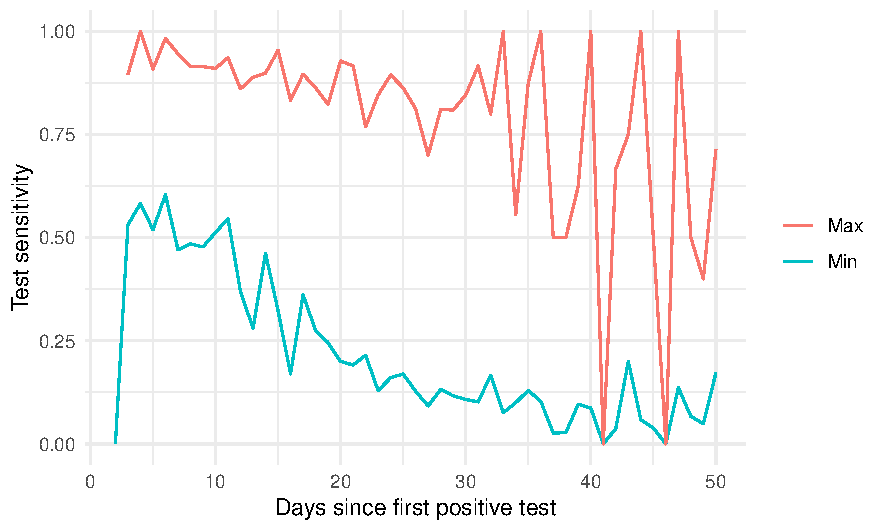
\includegraphics{cis-imperfect-testing/test-sens-bound}
  \caption[Bounding test sensitivity using CIS data]{
    Bounding the test sensitivity using CIS data as a function of time since the infection was detected.
  }
  \label{imperf-test:fig:bounding-cis-sensitivity}
\end{figure}

To assess the sensitivity of the procedure to a time-varying test sensitivity, it will be useful to simulate from a model with a varying test sensitivity as a function of days since the start of the infection episode.
Through consideration of \cref{imperf-test:fig:bounding-cis-sensitivity}, and the interaction of false negatives due to viral load in \cref{E-ATACCC}'s results, I propose the following model.
\begin{equation}
  p_\text{sens}(t) = \begin{cases}
    0.9 - \frac{0.9-0.5}{50}t &t \leq 50 \\
    0.5 &t > 50
  \end{cases}
  \label{imperf-test:eq:variable-test-sensitivity}
\end{equation}
where $t$ is the number of days since infection.
Therefore, this model consists of a linear decline in test sensitivity, before a constant minimum point.

This could be incorporated into the simulation study be generating test results at ...\todo{finish sentence}
Adapting the simulation study to incorporate this test sensitivity is much more similar to the data (see purple histogram in \cref{imperf-test:fig:sim-single-pos}).
This model does not require low test sensitivities early in the infection, maintaining compatibility with the results in \cref{E-ATACCC}.

\section{Likelihood modification for false negatives} \label{imperf-test:sec:modelling}

In this section, I introduce a simple model of false negatives (\ie allowing $\psens < 1$) into the likelihood derived in \cref{E-perf-test:sec:model}.
The simple model, including a constant test sensitivity, means the likelihood remains tractable.

First, in \cref{imperf-test:sec:modifying-p_ia}, I modify $p_{ia}$, the probability episode $i$ being admissible, to allow for the episode possibly being longer than observed.
Then, in \cref{imperf-test:sec:modifying-p_iu}, I modify $p_{iu}$, the probability episode $i$ being undetected, to allow for additional episodes being missed.

\subsection{Modifying \texorpdfstring{$p_{ia}$}{pia}} \label{imperf-test:sec:modifying-p_ia}

\todo[inline]{These definitions (up until next orange box) will move to chapter 2 where episodes are introduced}
The beginning of episode $i$ is known to occur in the interval $[l_i^{(b)}, r_i^{(b)}]$, and similarly for the end of the infection in $[l_i^{(e)}, r_i^{(e)}]$.

\todo[inline]{From here, this is the section's content}

I will modify $p_{ia}$ to allow the negative test following the last positive to be a false negative.
If it is a false negative, then I will consider the episode's end right-censored.
However, if it is a true negative, then the episode's end is interval-censored, as previously.
A mixture of these scenarios forms the episode's likelihood contribution, with the mixture probability determined by the test sensitivity.

I start by finding the tests that need consideration.
For tractability, assume that the negative test bounding the start of the infection, on day $l_i^{(b)}-1$, is a true negative.
This assumption is reasonable because the test sensitivity is high early in an infection; therefore, this test is unlikely to be a false negative.
For tractability and simplicity, I consider only tests between the positive tests providing a lower bound on the length of the episode.
By definition (see\todo{insert where these are defined in chapter 2}), these are the tests between $r_i^{(b)}$ and $l_i^{(e)}$ inclusive.
They are a subset of $\sched_i$, the set of test times for the individual in which episode $i$ occurs.
Denote this subset as $\sched'_i = \{ t \in \sched_i \ssep r_i^{(b)} \leq t \leq l_i^{(e)} \}$, and their results by $\vec{y_i'} = \{ y_i(t) \ssep t \in \sched'_i \}$ where $y_i(t) = 1$ if the test on day $t$ is positive and 0 otherwise.
As I assume that there are no false positives, the infection episode must span at least this period because it starts and ends with a positive test.
Therefore, the test results at times in $\sched_i'$ are either true positives or false negatives.

Now consider the negative test at $r_i^{(e)}+1$, the first negative after the start of the episode which may be a false negative.
It is a false negative if and only if the episode ends after the test, \ie $e_i > r_i^{(e)}$.
I proceed by considering whether this is the case, and considering the case with $b_i$ known; $b_i$ will later be integrated out.

First, if $e_i \leq r_i^{(e)}$, meaning that the test at $r_i^{(e)}+1$ is a true negative and the end of the episode is interval-censored as in the previous chapter.
In this case, the test at $r_i^{(e)} + 1$ is a true negative, as are all other tests not in $\sched'_i$.
These occur with probability 1, by the assumption of no false positives.
The tests in $\sched_i'$ are either true positives or false negatives.
\begin{align}
&p(\vec{y_i'}, e_i \leq r_i^{(e)} | b_i, p_\text{sens}, \theta) \\
&= p(\vec{y_i'}, l_i^{(e)} \leq e_i \leq r_i^{(e)} | t_i, b_i, p_\text{sens}, \theta) \\ % &\text{as no false positives}
&= p(\vec{y_i'} \mid l_i^{(e)} \leq e_i \leq r_i^{(e)}, t_i, b_i, p_\text{sens}, \theta) p(l_i^{(e)} \leq e_i \leq r_i^{(e)} | t_i, b_i, p_\text{sens}, \theta) \\
&= \left( \prod_{t \in \sched'_i} p_\text{sens}^{y_i(t)} (1 - p_\text{sens})^{(1 - y_i(t))} \right) \left( S_\theta(l_i^{(e)} - b_i - 1) - S_\theta(r_i^{(e)} - b_i - 1) \right)
\label{imperf-test:eq:ll-ei-lt-ri}
\end{align}

Second, if $e_i > r_i^{(e)}$.
In this case, the test at $r_i^{(e)}$ is a false negative, occurring with probability $(1 - p_\text{sens})$.
To avoid having to consider tests after $r_i^{(e)}$, which could greatly complicate the likelihood, I model this case as the episode being right-censored at $r_i^{(e)}$.
\todo{check previous notes - I think I investigated this assumption a bit more and maybe did some sensitivity analysis}
Taking the same approach as before:
\begin{align}
&p(\vec{y_i'}, e_i > r_i^{(e)} | b_i, p_\text{sens}, \theta) \\
&= p(y_i \mid e_i > r_i^{(e)}, t_i, b_i, p_\text{sens}, \theta) p(e_i > r_i^{(e)} | t_i, b_i, p_\text{sens}, \theta) \\
&= \left( \prod_{t \in \sched'_i} p_\text{sens}^{y_i(t)} (1 - p_\text{sens})^{(1 - y_i(t))} \right) (1 - p_\text{sens}) S_\theta(r_i^{(e)} - b_i - 1)
\label{imperf-test:eq:ll-ei-gt-ri}
\end{align}

These expressions can now be used to form the full replacement for $p_{ia}$, $p'_{ia}$, the likelihood of the data $\vec{y_i'}$.
First, augment the data with $b_i$, and split into the cases just discussed:
\begin{align}
p_{ia}'
&= p(\vec{y_i'} \mid p_\text{sens}, \theta) \\
&= \sum_{b_i = l_i^{(b)}}^{r_i^{(b)}} \left( p(\vec{y_i'}, e_i \leq r_i^{(e)} \mid b_i, p_\text{sens}, \theta) + p(\vec{y_i'}, e_i > r_i^{(e)} \mid b_i, p_\text{sens}, \theta) \right) p(b_i \mid p_\text{sens}, \theta).
\intertext{Now, substitute in \cref{imperf-test:eq:ll-ei-lt-ri,imperf-test:eq:ll-ei-gt-ri}, then take out the common factor:}
&= \left( \prod_{t \in \sched'_i} p_\text{sens}^{y_i(t)} (1 - p_\text{sens})^{(1 - y_i(t))} \right) \\ & \ \times \sum_{b_i = l_i^{(b)}}^{r_i^{(b)}} \left( S_\theta(l_i^{(e)} - b_i - 1) - S_\theta(r_i^{(e)} - b_i - 1) + (1 - p_\text{sens}) S_\theta(r_i^{(e)} - b_i - 1) \right) \\ & \ \times p(b_i \mid p_\text{sens}, \theta).
\intertext{This simplifies to:}
&= \left( \prod_{t \in \sched'_i} p_\text{sens}^{y_i(t)} (1 - p_\text{sens})^{(1 - y_i(t))} \right) \\ & \ \times \sum_{b_i = l_i^{(b)}}^{r_i^{(b)}} \left( S_\theta(l_i^{(e)} - b_i - 1) - p_\text{sens} S_\theta(r_i^{(e)} - b_i - 1) \right) p(b_i \mid p_\text{sens}, \theta).
\label{imperf-test:eq:pia-prime}
\end{align}
Note that if $p_\text{sens} = 1$ then $p_{ia}' = p_{ia}$.

Constant terms => proprtional to simpler thing

\subsection{Modifying \texorpdfstring{$p_{iu}$}{piu}} \label{imperf-test:sec:modifying-p_iu}

Several mechanisms for episodes being undetected were considered when deriving $p_{iu}$ in \cref{E-perf-test:eq:piu}.
I now consider the additional mechanisms arising due to false negatives.
Specifically, episode $i$ could be undetected if the first test after the $b_i$, episode $i$'s start day, is a false negative and then there are no subsequent positive tests.

This false negative would occur at the first test after the infection episode begins, on day $b_i + \tau_{\sched_i}(b_i)$ (see \cref{E-perf-test:sec:model}).
A false negative occurring requires that the episode has not yet ended but a negative still occurs.
The episode has not yet ended at the time of the test if $e_i = b_i + d_i - 1$ is after the test, that is the duration of the infection $d_i > \tau_{\sched_i}(b_i)$.
Conditional on the episode having not yet ended, the test result is negative with probability $1 - \psens$.

For there to be no subsequent positive tests, all tests up until day $e_i$ are false negatives.
I assume there is a negligible probability of two false negatives.
Therefore, this can only occur if the episode ends before another test.
Denote the number of days between $b_i$ and the test following the false negative as $\tau^2_{\sched_i}(b_i) \stackrel{\text{def}}{=} \tau_{\sched_i}(\tau_{\sched_i}(b_i) + 1)$.
Then, the episode ends before this test if $d_i < \tau^2_{\sched_i}(b_i)$.

Therefore, this mechanism causes episode $i$ to be undetected if all the following conditions hold.
\begin{enumerate}
    \item The episode would have been detected considering only the mechanisms in \cref{E-perf-test:eq:piu}. That is $b_i > \min(\sched_i)$ and $\tau_{\sched_i}(b_i) + b_i \leq e_i$.
    \item The episode ends in the interval $[\tau_{\sched_i}(b_i) + b_i, \tau^2_{\sched_i}(b_i) + b_i]$.
      Note that the lower bound here is exactly the bound on $e_i$ in the previous condition.
      Equivalently, $\tau_{\sched_i}(b_i) + 1 \leq d_i \leq \tau^2_{\sched_i}(b_i) + 1$.
    \item A false negative occurs on day $\tau_{\sched_i}(b_i) + b_i$. Conditional on the previous condition, this occurs with probability $1 - \psens$.
\end{enumerate}

The probability of this occurring, conditional on $B_i = b_i > \min(\sched_i)$ is:
\begin{align}
&\prob \left(
    \tau_{\sched_i}(b_i) + 1 \leq D_i \leq \tau^2_{\sched_i}(b_i) + 1
    \mid b_i,
\theta \right) (1 - \psens) \\
&= \left( S_\theta(\tau_{\sched_i}(b_i) + 1) - S_\theta(\tau^2_{\sched_i}(b_i) + 1) \right) (1 - \psens).
\end{align}
Integrating over $b_i$ for $\min \sched_i < b_i \leq T$ ($T$ being the last day of the period considered), in the same way as \cref{E-perf-test:eq:piu}, gives:
\begin{align}
\eta = (1 - p_\text{sens})\frac{1}{T} \sum_{b=\min(\sched_i) + 1}^T \left( S_\theta(\tau_{\sched_i}(b) + 1) - S_\theta(\tau^2_{\sched_i}(b) + 1) \right).
\end{align}

Denote the replacement for $p_{iu}$ as $p_{iu}'$.
$p_{iu}'$ is the probability of episode $i$ being missed, considering both the mechanisms from \cref{E-perf-test} and the new mechanism here.
These mechanisms are mutually exclusive.
Hence, $p_{iu}'$ is the sum of these, $p_{iu}' = p_{iu} + \eta$.
For the posterior density, \cref{E-perf-test:eq:full-posterior}, $1 - p_{iu}'$ is the required quantity.
\begin{align}
1 - p_{iu}'
&= 1 - p_{iu} - (1 - p_\text{sens})\frac{1}{T} \sum_{b=\min(\sched_i) + 1}^T \left( S_\theta(\tau_{\sched_i}(b) + 1) - S_\theta(\tau^2_{\sched_i}(b) + 1) \right) \\
&= \frac{1}{T} \sum_{b=\min(\sched_i) + 1}^T \left( p_\text{sens} S_\theta(\tau_{\sched_i}(b) + 1) + (1 - p_\text{sens}) S_\theta(\tau^2_{\sched_i}(b) + 1)\right).
\label{imperf-test:eq:pit-prime}
\end{align}

$p_{iu}'$ and $p_{ia}'$ are substituted for $p_{iu}$ and $p_{ia}$ respectively in \cref{E-perf-test:eq:full-posterior}.
The posterior density is otherwise unchanged.

\section{Simulation study} \label{imperf-test:sec:sim-study-results}

Here, I modify the simulation study in \cref{E-perf-test:sec:simulation-study} to assess several features of the statistical model I proposed in the previous section.
First, the ability to identify the survival function even with false negatives.
Second, the impact of misspecifying $\psens$, including violating the assumption that is constant.
Finally, the impact of the simplifying assumptions made in \cref{imperf-test:sec:modelling} for tractability.
These assumptions are that the previous negative is a true negative and that there is a negligible probability of missing an episode due to two false negatives.

I simulate datasets under four conditions: a constant $\psens$ of 0.6, 0.8, or 1.0 (the latter being the same as the simulated data in \cref{E-perf-test:sec:simulation-study}), or the varying test sensitivity model proposed at the end of \cref{imperf-test:sec:simulate}.
The simulation is otherwise unchanged from that in \cref{E-perf-test:sec:simulation-study}.
The number of single positive episodes in each of these conditions, compared to the number observed in the CIS data, is shown in \cref{imperf-test:fig:sim-single-pos}.

For each simulated dataset, I estimate the survival function using the likelihood proposed in \cref{imperf-test:sec:modelling} and assuming $\psens$ equals 0.6, 0.8, or 1.0.
If the dataset was simulated using a constant $\psens$, and that value of $\psens$ matches the value assumed during inference, I refer to $\psens$ as being correctly specified; otherwise I refer to it as misspecified.
However, there is still some misspecification of the model to false negatives owing to the simplifying assumptions made.
The amount that the simplifying assumptions are violated increases as $\psens$ decreases.

I use either the independent (vague) or model combination priors for the survival (described in \cref{E-perf-test:sec:parameters-priors}).
These were shown to be the best performing priors in \cref{E-perf-test:sec:results}.
Therefore, there are a total of 24 possible scenarios (each combination of: 4 simulated datasets, 3 values of $\psens$ in inference, and 2 priors), although not all are shown.

When $\psens = 0.8$ and is correctly specified, the model recovers the true survival time well (see \cref{imperf-test:fig:constant-test-sensitivity}(B)).
The informative prior, in comparison to the vague prior, helps to overcome the misspecification due to the simplifying assumptions, moving the estimated survival function closer to its true survival time.
However, when $\psens = 0.6$, this is no longer the case (see \cref{imperf-test:fig:constant-test-sensitivity}(A)).
This is likely caused by too large a violation of the simplifying assumptions made in \cref{imperf-test:sec:modelling}.
\begin{figure}
  % \makebox[\textwidth][c]{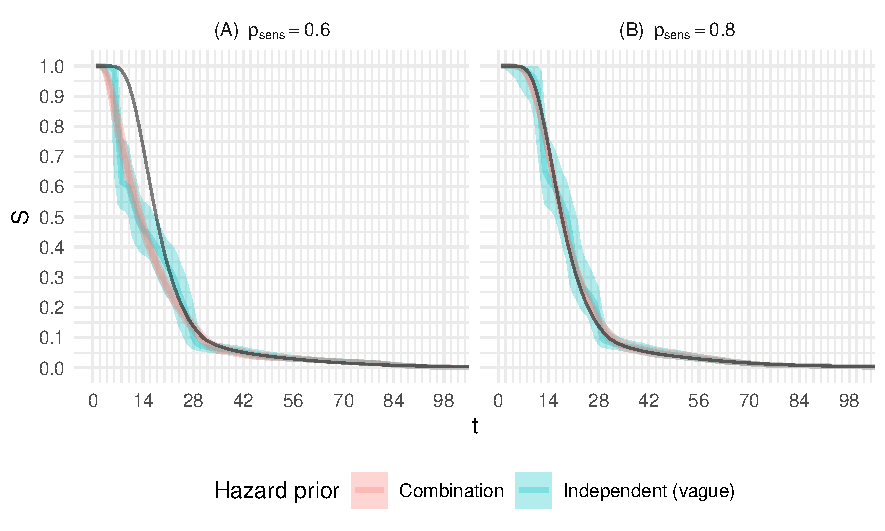
\includegraphics[width=1.2\textwidth]{cis-imperfect-testing/sim-constant-sensitivity}}
  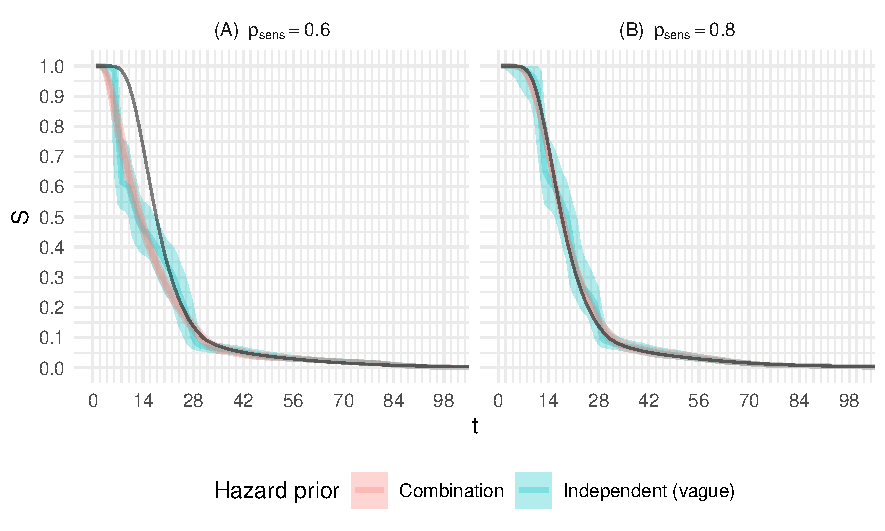
\includegraphics[width=\textwidth]{cis-imperfect-testing/sim-constant-sensitivity}
  \caption[Simulation study results with constant test sensitivity]{%
    Posterior (median and 95\% credible interval) of the survival time for the simulation study with a correctly specified test sensitivity.
    True survival time shown in black.
  }
  \label{imperf-test:fig:constant-test-sensitivity}
\end{figure}

If the test sensitivity is misspecified, that is the assumed value for $p_\text{sens}$ in \cref{imperf-test:eq:pit-prime,imperf-test:eq:pit-prime} is different to the value used in the simulation, then the survival time will be biased (see \cref{imperf-test:fig:misspecified-test-sensitivity}).
If $\psens$ is misspecified and too low (see \cref{imperf-test:fig:misspecified-test-sensitivity}(A)), then the posterior estimate initially follows the true value but then separates.
The number of episodes inferred to have truly ended by the first negative is too high, and hence the survival time is underestimated.
This affect dominates over the opposing bias of overestimating the number of missed episodes.
The opposite occurs if the test sensitivity is assumed to be too high, although the posterior moves away from the truth earlier (see \cref{imperf-test:fig:misspecified-test-sensitivity}(C)).
\begin{figure}
  % \makebox[\textwidth][c]{
    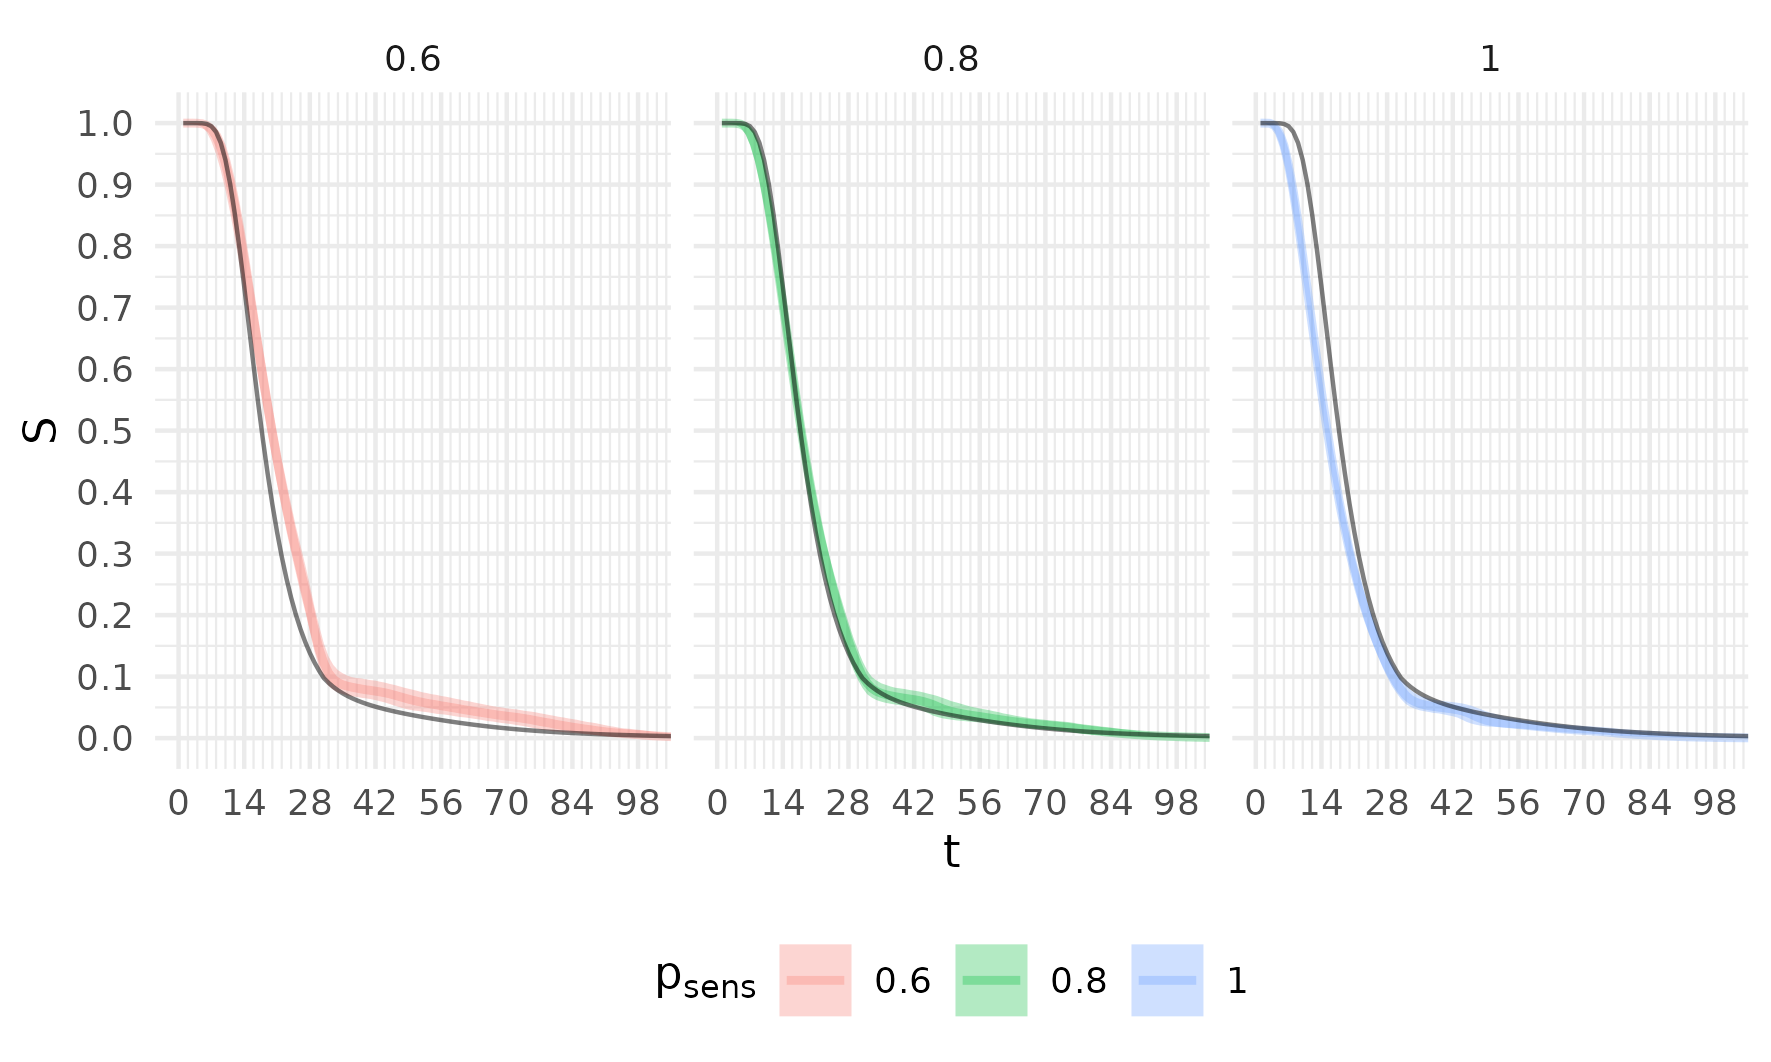
\includegraphics[width=\textwidth]{cis-imperfect-testing/sim-misspecified-sensitivity}
  \caption[Simulation study results with misspecified test sensitivity]{%
    Posterior (median and 95\% credible interval) of the survival time for the simulation study with a possibly misspecified test sensitivity.
    True survival time shown in black.
    All simulations use a constant test sensitivity of 0.8, but the inference procedure assumes different values, as per the key.
    Hence, (B) is correctly specified, and the same as in \cref{imperf-test:fig:constant-test-sensitivity}, but (A) and (C) have misspecified $\psens$.
    All results use the combination prior, due to it performing better than the vague prior in \cref{imperf-test:fig:constant-test-sensitivity}.
  }
  \label{imperf-test:fig:misspecified-test-sensitivity}
\end{figure}

The results when a varying test sensitivity (\cref{imperf-test:eq:variable-test-sensitivity}) is used for the simulation are similar to a constant 0.8 test sensitivity (see \cref{imperf-test:fig:variable-test-sensitivity}).
This suggests that the simplified model, with constant test sensitivity, is sufficient for recovering the true survival time.
Therefore, I will apply this model to the real CIS data in the next section.
\begin{figure}
  % \makebox[\textwidth][c]{
    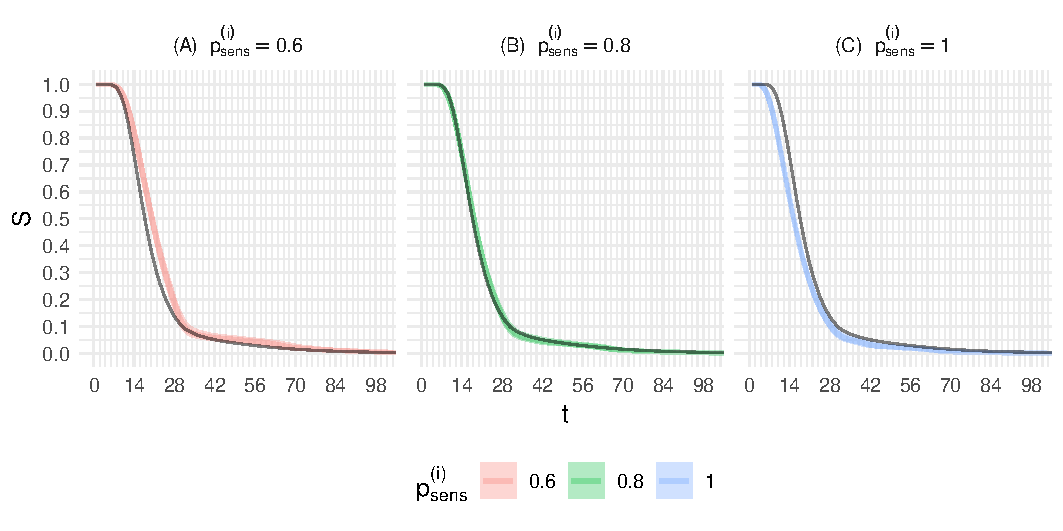
\includegraphics[width=\textwidth]{cis-imperfect-testing/sim-variable-sensitivity}
  \caption[Simulation study results with varying test sensitivity]{%
    Posterior (median and 95\% credible interval) of the survival time for the simulation study with a variable test sensitivity.
    Each panel shows the results of performing inference with a different assumed value for the test sensitivity.
    The posterior estimate using a model with a constant test sensitivity of 0.8 (B) is similar to the true value (black line).
  }
  \label{imperf-test:fig:variable-test-sensitivity}
\end{figure}

\section{Application to CIS data} \label{imperf-test:sec:application}

In this section I apply the approach described in this chapter to the CIS episodes dataset I described in \cref{E-perf-test:sec:approach}.
This is the 4,800 CIS infection episodes first detected between 10th Oct 2020 and 6th Dec 2020 inclusive and have negatives bounding the start and end time of the episode.

Unlike in the simulation studies, an uninformative prior on $\ntot$ led to implausible estimates of the duration distribution.
The uninformative prior led to high posterior estimates of $\ntot$, and hence an implausibly large number of episodes with durations of less than five days.
Therefore, I based an informative prior for $\ntot$ on pre-existing estimates of the total number of infections over the period with posterior mean \numprint{4136368} and standard deviation \numprint{27932}~\autocite{birrellRTM2}.
% This model gives a posterior mean of \numprint{4136368} cumulative infections in England in the time period I consider, with a posterior standard deviation of \numprint{27932}~\citePersonalComms{Paul Birrell}.
\todo{Insert correct citation for RTM paper 2 once available}
Approximating this distribution as a negative binomial and scaling the mean to the size of the CIS cohort gives the prior $\ntot \sim \NBc(\numprint{25132}, \numprint{22047})$ (distribution defined in \cref{E-distributions}).

With this prior, the model produces plausible estimates of the duration distribution (see \cref{imperf-test:fig:cis-estimates}).
This estimate has more long episodes than the estimate in \cref{E-ATACCC}.
The qualitative increase in long episodes is robust to the choice of prior for $\ntot$, the assumed value for $\psens$ (see \cref{imperf-test:fig:cis-sensitivity}), and the choice of prior for the hazard (see \cref{E-perf-test:sec:parameters-priors}), $\lambda$.
However, the survival proportion over the first 4 weeks is sensitive to these choices.
The estimate using a test sensitivity of 0.8 and $\NBc(\numprint{25132}, \numprint{22047})$ give a median survival time most similar to that of \cref{E-ATACCC}.
\begin{figure}
  \centering 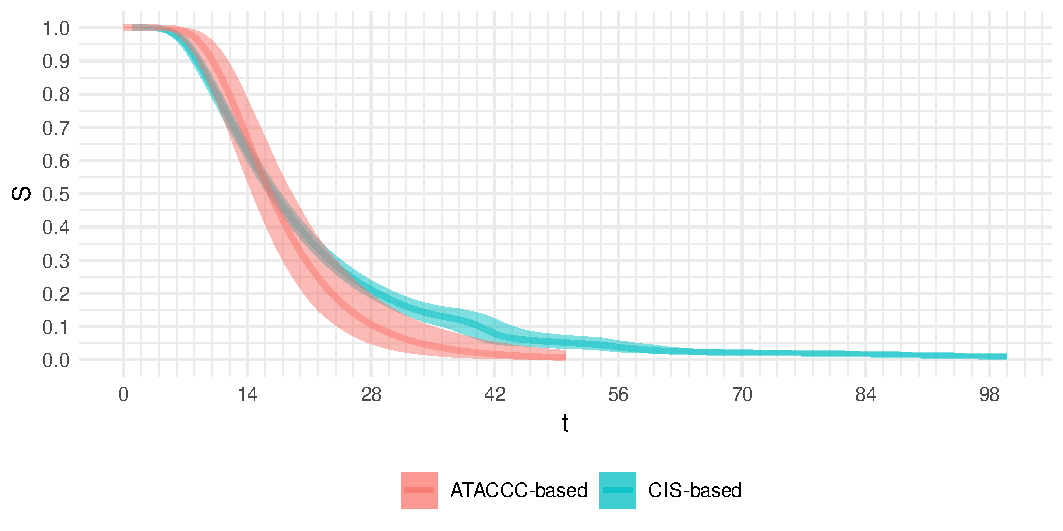
\includegraphics{cis-imperfect-testing/CIS_final}
  \caption{Duration estimates using CIS and ATACCC data}
  \label{imperf-test:fig:cis-estimates}
\end{figure}
\begin{figure}
  \vspace{-2.5cm}
  \makebox[\textwidth][c]{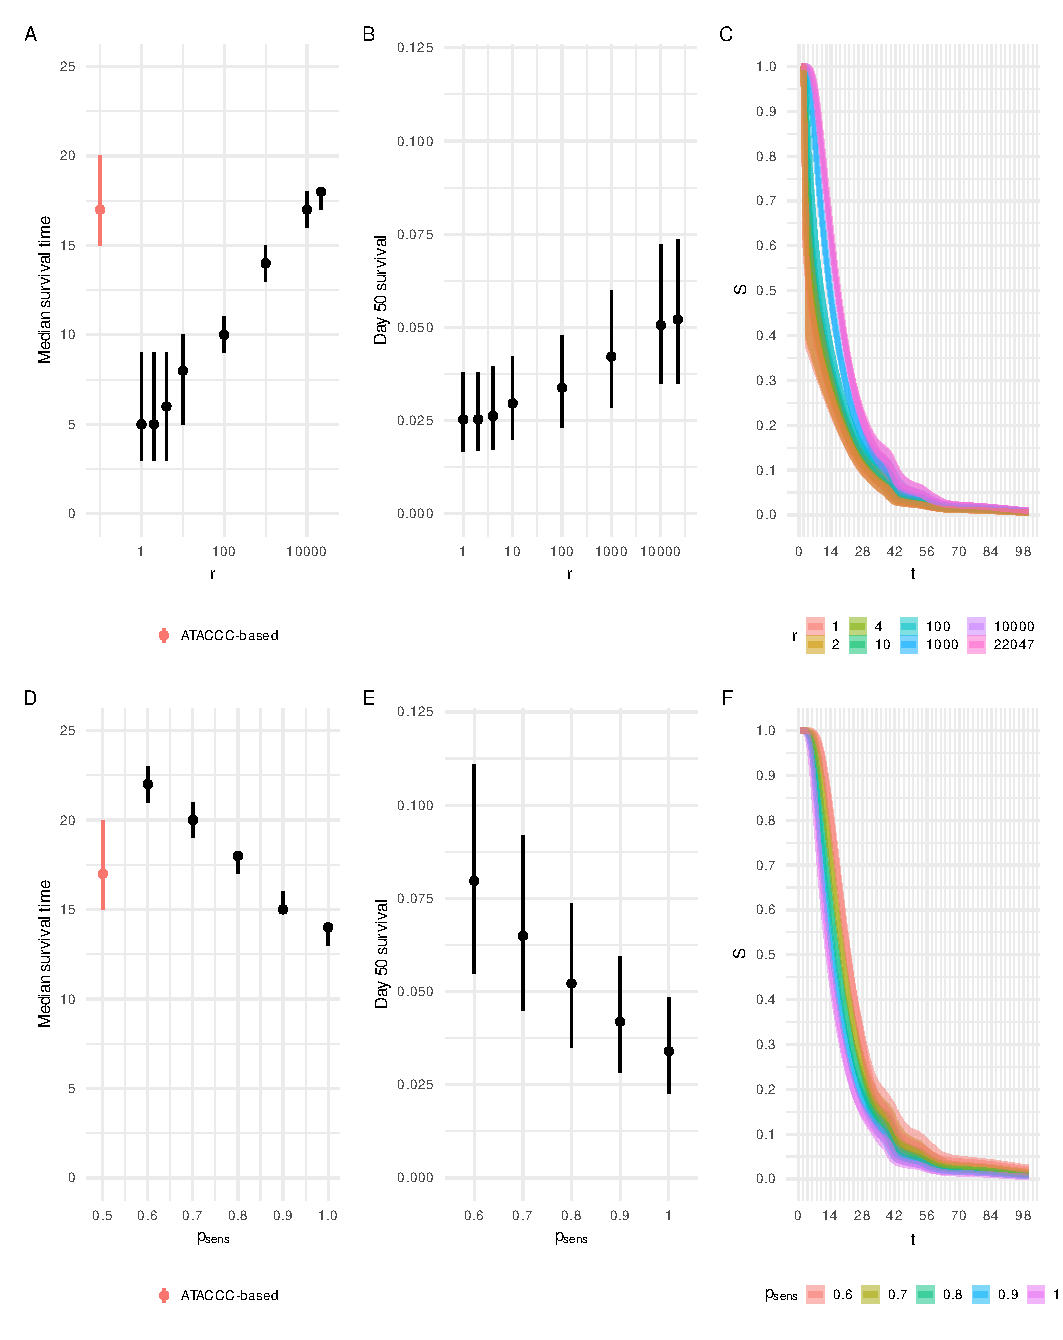
\includegraphics{cis-imperfect-testing/CIS_vary}}
  \caption{%
    Sensitivity of CIS estimates to: (A-C) the value of $r$, the dispersion of the prior for $\ntot$ (a larger $r$ means a more informative prior), and (D-F) $\psens$.
    A and D: median survival time, in comparison to the ATACCC-based estimate of \cref{E-ATACCC}.
    B and E: survival at day 50, $S_\theta(50)$.
    C and F: full survival curves out to day 100.
  }
  \label{imperf-test:fig:cis-sensitivity}
\end{figure}

The assumption that the estimates are most sensitive to is the strength of the prior on $\ntot$.
A very weak, almost uninformative, prior on this quantity causes the posterior estimate to be much higher than the estimate from \textcite{birrellRTM2}.
When increasing the prior's strength, the posterior estimate moves towards the prior smoothly, as expected (see \cref{imperf-test:fig:ntot}).
Taking a prior from \textcite{birrellRTM2} means that the posterior survival is close to the \cref{E-ATACCC} estimate in the region where that estimate is reliable.
This justifies the use of this prior.
\begin{figure}
  \centering 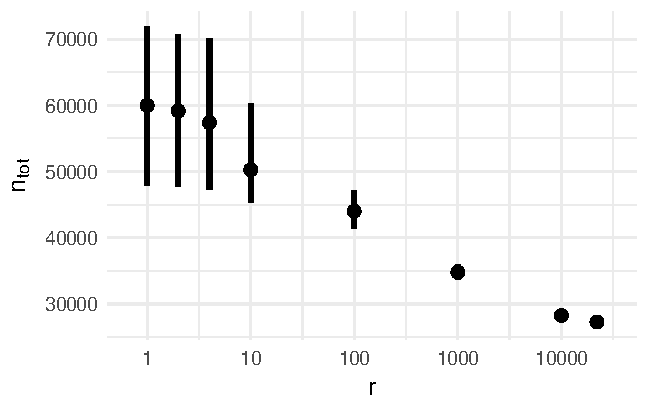
\includegraphics{cis-imperfect-testing/CIS_ntot}
  \caption{How the posterior estimate of $\ntot$ changes with the value of $r$ in the prior on $\ntot$.}
  \label{imperf-test:fig:ntot}
\end{figure}

\section{Discussion} \label{imperf-test:sec:discussion}

In this chapter, I developed a novel method to incorporate false negatives into the survival analysis of \cref{E-perf-test}.
I then applied this method to the CIS data, estimating the tail of the duration distribution without the strong model assumptions and extrapolation in \cref{E-ATACCC}.
The qualitative features of the estimated distribution are robust to the assumed value for $\psens$, and the choice of prior for $\lambda$, although the quantitative details are not.
The estimates of the tail, the primary purpose of this chapter, are in addition somewhat robust to the choice of prior for $\ntot$.
However, the rest of the distribution is sensitive to this choice.

An informative prior on $\ntot$ is required is for the bulk of the distribution to agree with those in \cref{E-ATACCC} and the wider literature.
In the simulation study, the uninformative prior on $\ntot$ performed well, even when the test sensitivity was misspecified.
A possible explanation is that the true variation in the test sensitivity is significantly different to the function in \cref{imperf-test:eq:variable-test-sensitivity}.
In particular, the test sensitivity for long episodes may become much lower than 50\%.
This allows many more episodes to be missed than the model assumes, and hence a higher $\ntot$ is required to explain the data.
Furthermore, it violates assumptions made in \cref{imperf-test:sec:modelling}; this is similar to when the simulating using a too low test sensitivity.
Violating these assumptions would lead to unpredictable inference results, perhaps those seen here.

Ideally, the test sensitivity would be estimated from the data.
However, this would require incorporating time-varying test sensitivity into the likelihood.
Furthermore, it is unclear that such a model would be identifiable because it would not be clear whether to attribute negative results to false negatives or to recoveries\todo{cite identifiability issues with varying sensitivity}.

The assumption, made in \cref{E-perf-test}, was that the episode start times are independent.
However, because infections are the result of a counting process with intensity shared between individuals (see \cref{E-inc-prev:sec:infection-process}), this assumption is violated.
Prevalence was fairly constant over the period I chose, suggesting the same is true of the incidence.
Additionally, some simulations exploring the results of changing incidence suggested this would not have a large effect on the results (not shown).

% However, comparing the CIS and simulated datasets do not show any differences which suggest what in the data is causing these differences.
% Then, the additional missed infections implied by a 
% This would lead to more missed infections than the model assumes, and hence a higher $\ntot$ is required to explain the data.

\section{Conclusion} \label{imperf-test:sec:conclusion}

In this chapter, I developed and applied novel methodology to estimate the duration distribution of RT-PCR-positivity using information from two studies: ATACCC and CIS.
Assuming a test sensitivity of 0.8 and an informative prior on the number of infections, provided the preferred estimates.

These estimates are the first estimates of the duration of RT-PCR-positivity, including the distribution tails, estimated from general population data.
This feature of the distribution is important for understanding the proportion of prevalence attributable to long infections and interpreting RT-PCR test results.
\todo{possibly cut some of this text?}
Producing these estimates required applying previous survival analysis frameworks in the novel context of the CIS.
The framework needed further modification to account for the presence of false negatives, done in this chapter.

The posterior distribution for the survival is concentrated, producing narrow credible intervals, likely due to the large sample size in the CIS.
In the following chapters, I will take the posterior mean for the survival time at each point, neglecting this uncertainty, as the basis for estimating transmission.
% First, I will take a backcalculation approach (\cref{E-backcalc}), based on the framework in \cref{E-inc-prev}.
% Then, I will take a mechanistic approach (\cref{E-SEIR}), modelling the transmission process explicitly.

\ifSubfilesClassLoaded{
  \listoftodos
}{}

\end{document}